\section{\large Аналитическая часть}

В данном разделе проводится анализ предметной области, анализ способов хранения данных в приложении и выбор оптимального, а также формализация требований к разрабатываемой программе.

Для анализа предметной области рассматриваются основные функции и задачи поликлиники, а также минимальный штат поликлиники. Для более точного анализа способов хранения данных в приложении предлагается рассмотреть классификацию СУБД по двум харатеристикам, модели хранения данных и по архитектуре организации данных.

\subsection{Анализ предметной области}

Поликлиникой будем называть многопрофильное лечебно-\linebreak профилактическое учреждение, оказывающее медицинскую помощь населению на закрепленной территории на догоспитальном этапе.

Основными функциями и задачами поликлиники являются:

\begin{itemize}[leftmargin=1.6\parindent]
	\item[---] оказание квалифицированной специализированной медицинской помощи населению непосредственно в поликлинике;
	\item[---] оказание первой медицинской помощи при острых заболеваниях, травмах, отравлениях и других неотложных состояниях независимо от места проживания больного;
	\item[---] своевременная госпитализация нуждающихся в стационарном лечении;
	\item[---] экспертиза временной нетрудоспособности, освобождение больных от работы, направление на медико-социальную экспертизу лиц с признаками стойкой утраты трудоспособности;
	\item[---] организация и проведение комплекса профилактических мероприятий, направленных на снижение заболеваемости, инвалидности и смертности среди населения, проживающего в районе обслуживания, а также среди работающих на прикрепленных предприятиях;
	\item[---] организация и осуществление диспансеризации населения (здоровых и больных);
	\item[---] организация и проведение мероприятий по санитарно-гигиеническому воспитанию населения, пропаганде здорового образа жизни.
\end{itemize}

Согласно рекомендации Минздрава России~\cite{minsdrav-state}, в штате поликлиники должно быть не менее 50 человек, однако, в случае частной поликлиники, это количество может быть уменьшено до следующих позиций:

\begin{enumerate}[label=\arabic*)]
	\item главный врач (1 должность);
	\item врачи специалисты (минимум 2 должности);
	\item уборщик (1 должность);
	\item системный администратор (1 должность).
\end{enumerate}



\subsection{Анализ способов хранения данных в приложении}

Рассмотрим понятия БД и СУБД и их основные функции, модели данных, а также способы классификации СУБД.

Классифицировать СУБД предлагается по модели хранения данных (дореляционные, реляционные и постреляционные), а также по архитектуре организации хранения данных (файл-серверные, клиент-серверные, встраиваемые и сервисо-ориентированные).

Также необходимо выбрать тип СУБД, с использованием которой будет осуществляться дальнейшая разработка.

\subsubsection{БД и СУБД}

База данных, сокращённо БД (\textit{англ.} DB --- database) \cite{carpova} --- совокупность структурированных взаимосвязанных данных, относящихся к определённой \linebreak предметной области и организованных таким образом, что эти данные могут быть использованы для решения многих задач многими пользователями.

Система управления базами данных, сокращённо СУБД (\textit{англ.} DBMS --- database management system)~\cite{carpova} --- программная система, предназначенная для создания на ЭВМ общей базы данных для множества приложений, поддержания её в актуальном состоянии и обеспечения эффективного доступа пользователей к содержащимся в ней данным в рамках предоставленных им полномочий. 

Основными функциями СУБД являются:
\begin{enumerate}[label=\arabic*)]
	\item управление данными во внешней памяти (обеспечение абстракции пользователя от организации данных);
	\item управление данными во внутренней памяти (обеспечение работы с буферами оперативной памяти);
	\item управление транзакциями (поддержка транзакций по принципу "всё или ничего", обеспечение их целостности);
	\item журнализация (возможность восстановить состояние после сбоя);
	\item поддержка языков БД (например, поддержка SQL).
\end{enumerate}


\subsubsection{Модели данных и способы классификации СУБД}

Моделью данных  (\textit{англ.} data model) \cite{carpova-t-s} называют абстракцию, которая, будучи приложима к
конкретным данным, позволяет пользователям и разработчикам трактовать их уже как информацию, то есть сведения, содержащие не только данные, но и взаимосвязь между ними. На рисунке~\ref{fig:data-models} приведена классификация моделей данных.

\begin{figure}[h]
	\centering
	\captionsetup{justification=centering}
	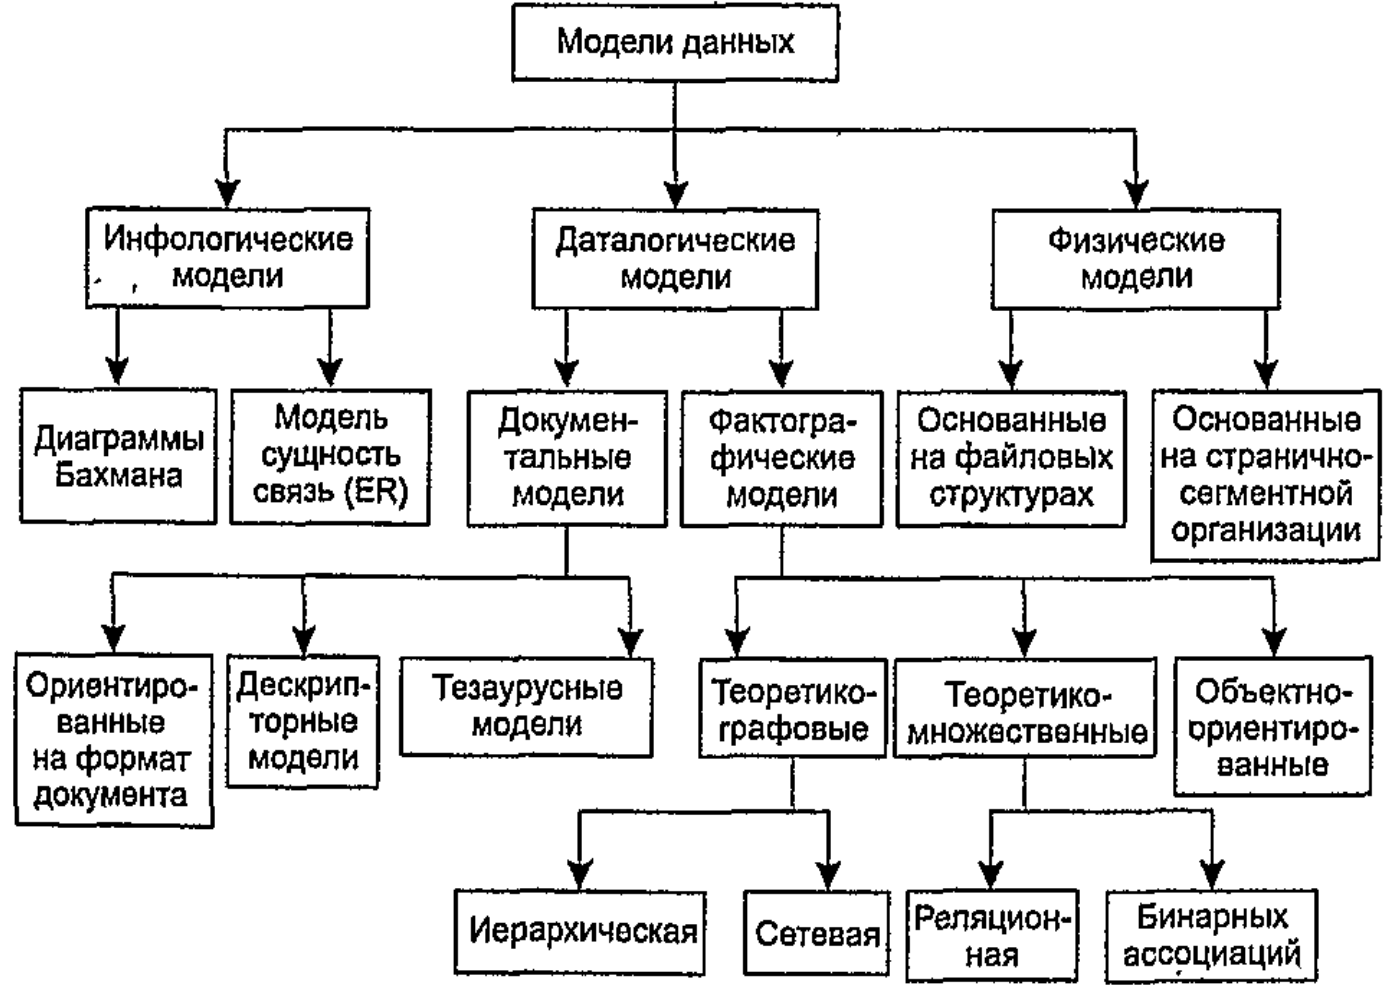
\includegraphics[width=140mm]{datamodels.png}
	\caption{Классификация моделей данных}
	\label{fig:data-models}
\end{figure}

Рассмотрим, как можно классифицировать существующие СУБД по двум харатеристикам: модели хранения данных и архитектуре организации хранения данных.

\subsubsection{Модели хранения данных}

По модели хранения данных выделяют следующие СУБД:

\begin{enumerate}[label=\arabic*)]
	\item дореляционные (инвертированые списки, иерархические и сетевые СУБД)
	\item реляционные;
	\item постреляционные.
\end{enumerate}

Системы, основанные на инвертированных списках (например, Datacom компании Applied Data Research, Inc.), поддерживают два типа операторов: прямые поисковые операторы (например, найти первую запись таблицы по некоторому пути доступа), а также операторы, находящие запись в терминах относительной позиции от предыдущей записи.
В таких СУБД отсутствуют общие правила определения целостности данных, а хранимые таблицы и пути доступа к ним видны всем пользователям,

Иерархические СУБД содержат упорядоченный набор деревьев, причём каждый тип дерева состоит из одной корневой записи и упорядоченного набора типов поддеревьев.
Для базы данных определяется полный порядок обхода деревьев --- например, сверху вниз и слева направо. 
Типичным представителем (наиболее известным и распространенным) является Information Management System (IMS) фирмы IBM.

Сетевые СУБД содержат наборы записей и связей между этими записями. 
Сети являются естественным способом представления отношений между объектами и всемозможными взаимосвязями между ними.
Сетевая модель опирается на математическую структуру направленного графа --- структуры, состоящей из узлов, соединённых направленными рёбрами (узлы представляют собой объекты в виде типов записей данных, а рёбра --- связи между объектами).
К известным сетевым системам управления базами данных относится: DBMS, IDMS, TOTAL, VISTA.

Реляционная модель данных (РМД) была предложена математиком Э.Ф. Коддом в 1970 г. 
РМД является наиболее широко распространенной моделью данных и единственной из трех основных моделей данных, для которой разработан теоретический базис с использованием теории множеств.

Основной структурой в РМД является отношение, вследствие чего и была называна модель (от \textit{англ.} relation --- отношение). 
Представление отношения может быть осуществлено в виде таблицы, а управление данными, которые связывают отношения, обеспечивается при помощи SQL --- декларативного языка структурированнных запросов (\textit{англ.} Structured Query Language), который основан на реляционной алгебре. 
Несмотря на наличие таких достоинств, как простота и популярность использования, реляционные СУБД имеют и недостатки, такие, как отсутствие специальных средств для отображения различных типов связей (например, ''многие ко многим'').

Примерами реляционных СУБД являются Oracle, Microsoft SQL Server, а также PostgreSQL.

\subsubsection{Архитектуры организации хранения данных}

По архитектуре организации хранения данных выделяют следующие \linebreak СУБД:

\begin{enumerate}[label=\arabic*)]
	\item файл-серверные;
	\item клиент-серверные;
	\item встраиваемые;
	\item сервисно-ориентированные;
	\item прочие (временные, пространственные, пространственно-временные).
\end{enumerate}

При файл-серверной организации хранения данных система не имеет сетевого разделения компонентов диалога и использует файловую систему компьютера для отображения. 
Это облегчает нагрузку на центральный процессор (поскольку файл-сервер лишь извлекает данные из файлов), но добавляет нагрузку на сеть, что является существенным недостатком таких систем.
Примерами  файл-серверных СУБД являются  Microsoft Access и MySQL (до версии 5.0).

Клиент-серверные СУБД состоят из двух частей: клиентской части (которая включена в прикладную программу) и непосредственно сервера, являющегося внешней по отношению к клиенту программой. Преимущества данной системы:
\begin{itemize}[leftmargin=1.6\parindent]
	\item[---] возможность по мере надобности заменить один сервер другим;
	\item[---] обеспечивание разграничения доступа между пользователями;
	\item[---] снижение нагрузки на сеть и на клиентские машины.
\end{itemize}

Недостатком клиент-серверных СУБД является само существование сервера (это плохо для локальных программ) и количество вычислительных ресурсов, потребляемых сервером.
Клиент-серверными СУБД являются, например, Oracle, Microsoft MySQL Server, PostgreSQL, а также MySQL (версии 5.0 и выше).

Встраиваемой СУБД называют СУБД, тесно связанную с прикладной программой и работающую на том же компьютере, не требуя профессионального администрирования. 
Благодаря непосредственной близости данных к прикладной области, встраиваемые СУБД применяются в программах, которые хранят большие объёмы даннных, но в которых не требуется доступ с многих компьютеров.
Встраиваемыми системами являются SQLite, Firebird Embedded, Microsoft SQL Server Compact.


\subsubsection{Выбор типа СУБД}

По модели хранения данных будет выбрана реляционная модель, поскольку её популярность и универсальность (согласно списку самых популярных СУБД на декабрь 2023 года, 4 самых популярных СУБД являются реляционными~\cite{db-engine}) сделали её наиболее подходящей для использования в системах представления знаний, чем другие системы.

По архитектуре организации хранения данных будет выбрана \newline клиент-серверная СУБД, поскольку из предметной области следует требование к доступу к данным с многих компьютеров, а также достаточная скорость работы системы при малой нагрузке сети.

\subsection{Группы пользователей}

Выделим группы пользователей разрабатываемой системы, исходя из \linebreak предметной области поставленной задачи.

Выделяется 4 типа пользователей: системный администратор, главный врач, врач и работник регистратуры.
Предусмотрим набор возможностей для каждого типа пользователей.

Набор возможностей системного администратора:
\begin{itemize}[leftmargin=1.6\parindent]
	\item[---] вход в систему;
	\item[---] регистрация новых пользователей;
	\item[---] настройка уровней доступа.
\end{itemize}

Набор возможностей главного врача:
\begin{itemize}[leftmargin=1.6\parindent]
	\item[---] вход в систему;
	\item[---] учёт пациента;
	\item[---] учёт сотрудника;
	\item[---] просмотр расписания врачей и кабинетов.
\end{itemize}

Набор возможностей врача:
\begin{itemize}[leftmargin=1.6\parindent]
	\item[---] вход в систему;
	\item[---] приём пациента;
	\item[---] управление электронной медицинской картой пациента;
	\item[---] просмотр расписания врачей и кабинетов.
\end{itemize}

Набор возможностей работника регистратуры:
\begin{itemize}[leftmargin=1.6\parindent]
	\item[---] вход в систему;
	\item[---] регистрация нового пациента;
	\item[---] учёт пациента;
	\item[---] просмотр расписания врачей и кабинетов.
\end{itemize}

Данные наборы возможностей сотрудников поликлиники можно объединить в диаграмму, приведённую на рисунке~\ref{fig:usecase}.

\begin{figure}[h!]
	\centering
	\captionsetup{justification=centering}
	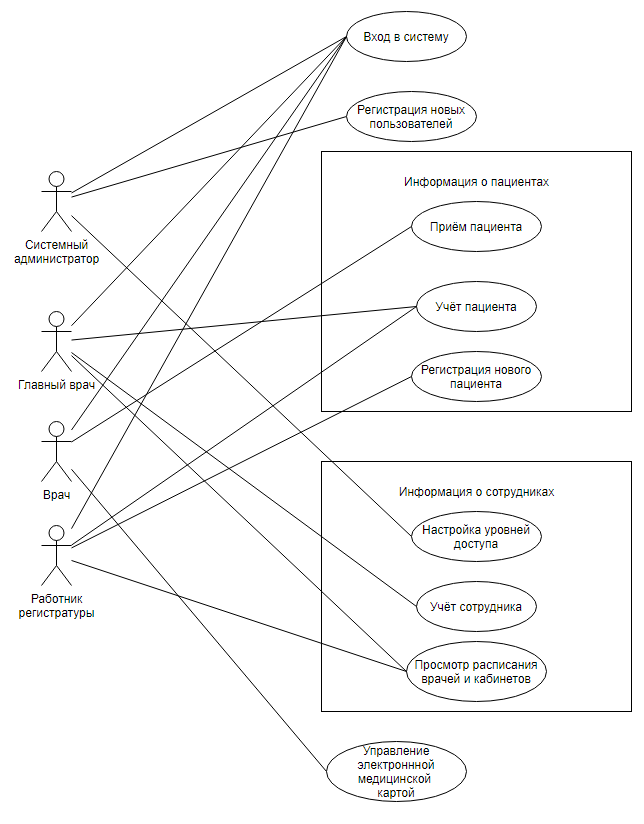
\includegraphics[width=150mm]{usecase.png}
	\caption{Диаграмма вариантов использования для поставленной предметной области}
	\label{fig:usecase}
\end{figure}


%\subsection{Структура базы данных}
%
%Для определения структуры базы данных необходимо на основе заданной предметной области определить категории данных, с которыми будет осуществлятья работа, определить информацию, которую будет содержать каждая категория, а также построить ER-диаграмму на основе полученных данных.

\subsection{Категории данных}

Основываясь на анализе предметной области, можно выделить следующие категории данных:
\begin{itemize}[leftmargin=1.6\parindent]
	\item[---] пользователь системы;
	\item[---] пациент поликлиники;
	\item[---] сотрудник поликлиники;
	\item[---] должность в поликлинике;
	\item[---] приём пациента;
	\item[---] расписание;
	\item[---] медицинская карта пациента;
	\item[---] состояние пациента;
	\item[---] договор с пациентом;
	\item[---] паспорт;
	\item[---] адрес.
\end{itemize}

Информация, соответствующая каждой категории, содержится в таблице~\ref{table:category-info}.

\clearpage

\begin{table}[H]
\begin{center}
	\captionsetup{justification=raggedright,singlelinecheck=off,margin=5mm}
	\caption{Информация для выделенных категорий данных}
	\begin{tabular}{| c | c |}
		\hline
		Категория данных & Информация \\
		\hline
		Пользователь системы & логин, пароль, сотрудник, уровень доступа \\
		\hline
		Пациент поликлиники & \makecell{паспорт, адрес, телефон,\\ домашний телефон, почта}  \\
		\hline
		Сотрудник поликлиники & \makecell{паспорт, должность, \\дата наёма, дата увольнения} \\
		\hline
		Должность в поликлиники & название должности, зарплата \\
		\hline
		Приём пациента & 
\makecell{врач, пациент, дата, \\
	динамика состояния, назначение,\\
	примечание, состояние}\\
		\hline
		Расписание &\makecell{сотрудник, день недели, кабинет, \\
время начала работы, время \\окончания работы}\\
		\hline
		Медицинская карта пациента & паспорт, договор, дата постановки на учёт \\
		\hline
		Состояние пациента & \makecell{общее состояние, рост,\\ вес, пульс, давление, \\температура, прочее }\\
		\hline
		Договор с пациентом & \makecell{номер договора, пациент, \\дата заключения, дата \\окончания, дата обновления} \\
		\hline
		Паспорт & \makecell{фамилия, имя, отчество, \\
дата рождения, пол, серия, \\
номер, дата выдачи, место выдачи} \\
		\hline
		Адрес & страна, город, улица, дом, этаж, квартира \\
		\hline
	\end{tabular}
	\label{table:category-info}
\end{center}
\end{table}

\subsection{Формализация задачи}

При помощи диаграммы сущность-связь (\textit{англ.} entity-relation diagram) можно выделить ключевые сущности, их атрибуты, а также типы и род связей между этими сущностями.
На основе даанных связей позже будет построоена диаграмма базы данных, поскольку связи между сущностями поозволяют точнее определить связи между объектами базы данных.
Диаграмма сущность-связь для поставленной предметной области приведена на рисунке~\ref{fig:er}.

\begin{figure}[h!]
	\centering
	\captionsetup{justification=centering}
	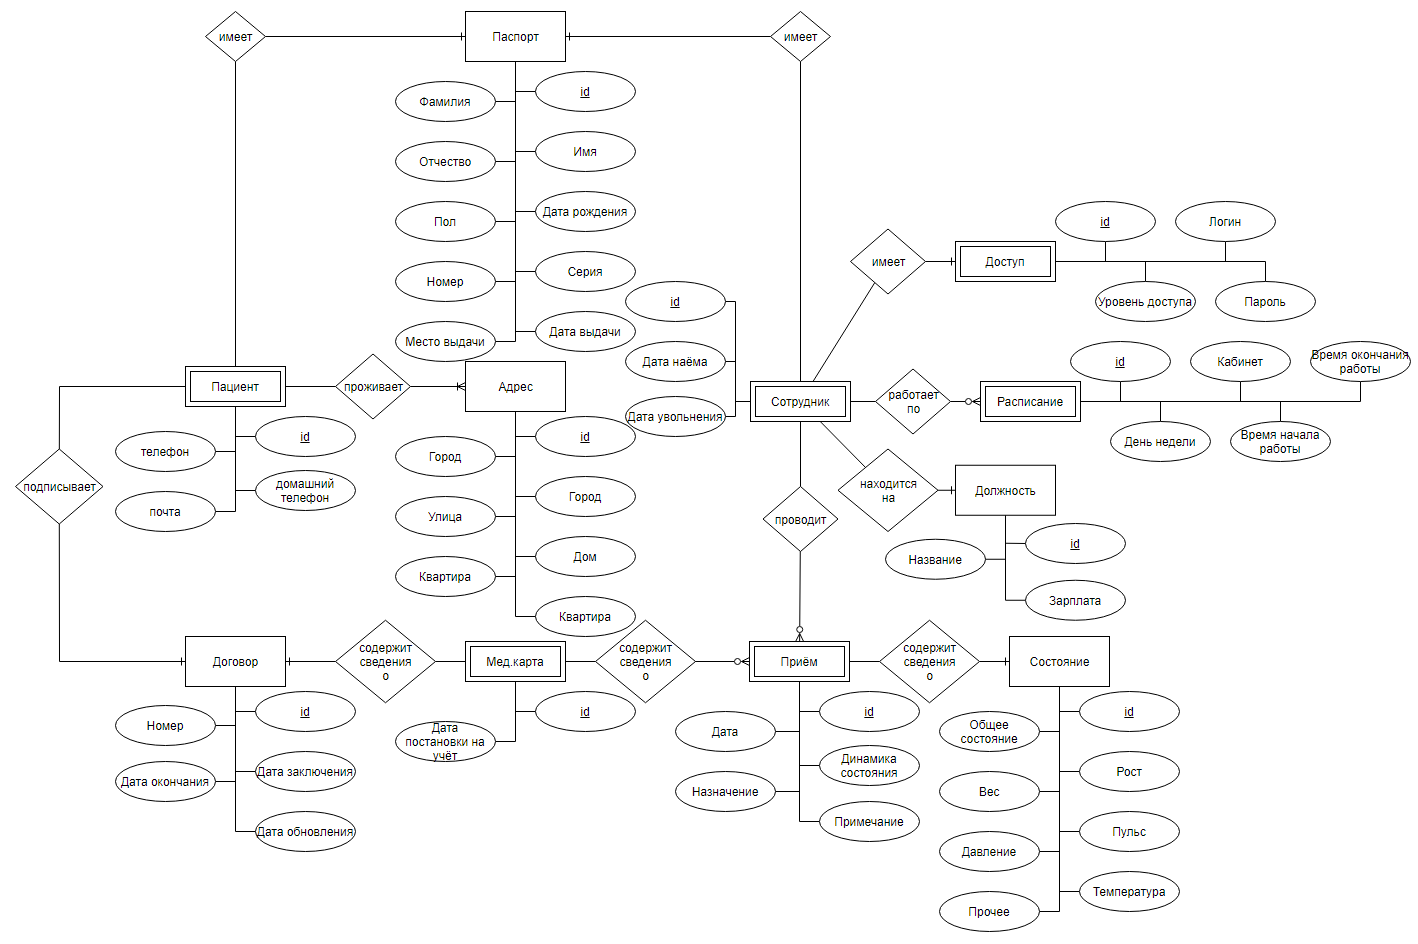
\includegraphics[angle=90, width=150mm]{er.png}
	\caption{Диаграмма сущность-связь для поставленной предметной области}
	\label{fig:er}
\end{figure}


%\subsection{Общий вид архитектуры}
%
%Выбрав СУБД, которая будет использована для разработки, на основе анализа поставленной задачи опишем общий вид реализуемой архитектуры.
%
%Архитектура программного обеспечения (\textit{англ.} software architecture)~\cite{clean-architecture} --- это форма, которая придаётся системе с целью упрощения разработки, развёртывания и сопровождения. 
%
%Для выбранной системы организации данных подходит клиент-серверная двузвенная архитектура (\textit{англ.} client-server tw-tier architecture)~\cite{client-server}, согласно которой сервер (процесс, реализующий некоторые сервисы, например, базу даных) предоставляет ресурсы набору соединённых с ним клиентов (процессы, запрашивающие сервисы у серверов путём посылки запроса и последующего получения ответа).
%Таким образом, совокупность клиентов и серверов вместе с промеждуточным программным обеспечение образуют единую систему, которая позволяет выполнять анализ и использование представленных данных.
%
%В двузвенной архитектуре клиент и сервер могут как находиться на одной машине, так и на разных. 
%Это обеспечивает сохранность и целостность данных, а также  упрощает поддержку многопользовательского режима работы с общими данными.
%
%Недостатком данной архитектуры является большой расход на поддержание работы приложений на рабочих станциях клиентов, что может существенно усложнить администрирование в больших системах.
%Тем не менее, для выбранной предметной области количество клиентов будет небольшим: рекомендованное Минздравом~\cite{minsdrav-state} количество должностей в поликлинике (55) является небольшим относительно того, какое количество клиентов обслуживают, например, современные социальные сети (согласно отчёту социальной сети ВКонтакте~\cite{vk-results}, количество российскийх пользователей в месяц составляет 73.4 млн. человек).
%
%Диаграмма работы двухзвенной клиент-серверной архитектуры с сервером СУБД приведён на рисунке~\ref{fig:client-server}.
%
%
%\begin{figure}[h!]
%	\centering
%	\captionsetup{justification=centering}
%	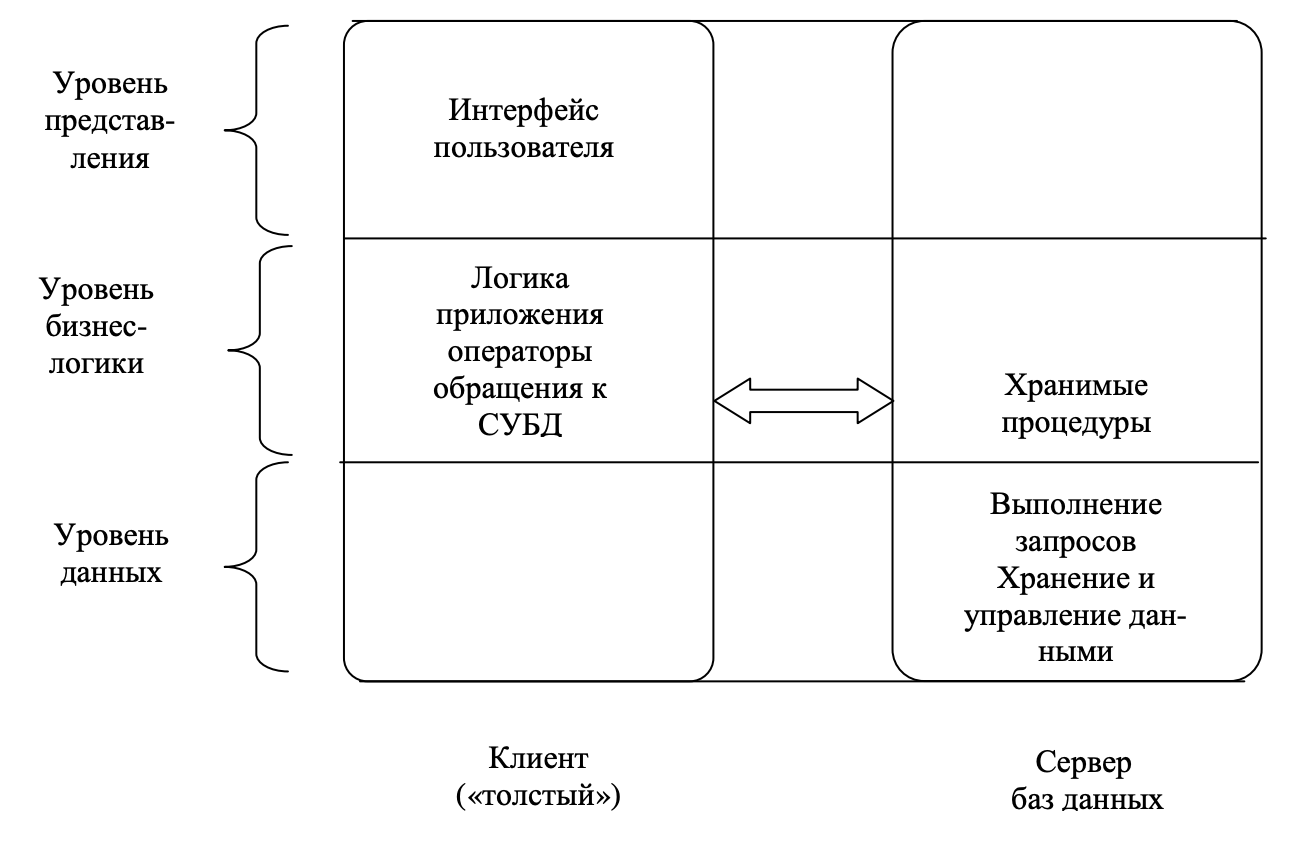
\includegraphics[width=100mm]{client-server.png}
%	\caption{Диаграмма двузвенной клиент-серверной архитектуры}
%	\label{fig:client-server}
%\end{figure}

\subsection*{Вывод}
В данном разделе был проведён анализ предметной области (информационные системы для частных поликлиник), а также проведён анализ существующих СУБД. 
Как СУБД, при помощи которой будет решаться поставленная задача, была выбрана реляционная клиент-серверная СУБД PostgreSQL
%Как архитектуру разрабатываемой информационной системы была выбрана двузвенная клиент-серверная архитектура. 
Были приведены диаграммы сценариев использования информационной системы, проанализированы категории даных, приведена диаграмма сущность-связь, поясняющая суть связей между выделенными сущностями, соответствующими категориям данных.


